\documentclass{ctexart}
\usepackage{graphicx}
\usepackage{amsmath}
\usepackage{amssymb}
\usepackage{hyperref}
\usepackage{geometry}
\usepackage{enumitem}
\geometry{a4paper, left=1in, right=1in, top=1in, bottom=1in}

\title{《深度学习基础》第二次实验报告}
\author{PB24000150 李欣宸}
\date{\today}

\begin{document}

\maketitle

本文是《深度学习基础》第二次实验报告。代码实现主要在 \verb|load.ipynb| 与 \verb|cnn.py| 中；其中 notebook 里定义了统一的 \verb|train_model| 实验入口，用于完成四组对比实验、测试集评估、混淆矩阵与错分样本分析。

\section{实验设置}

\paragraph{数据集}
本实验使用 Fashion-MNIST 数据集，共包含 60000 张训练图像和 10000 张测试图像，图像大小为 $28 \times 28$，均为单通道灰度图。训练前对输入进行了标准化处理，所用均值和标准差分别为 0.2860 与 0.3530。

\paragraph{数据划分}
将原始训练集按 $5:1$ 划分为训练集与验证集，即 50000 张训练图像与 10000 张验证图像；测试集保持官方划分不变。训练与验证阶段均采用批量大小 512。

\paragraph{基线模型}
基线模型采用 3 层卷积结构，通道数依次为 $32 \rightarrow 64 \rightarrow 128$，前两层后接池化层，卷积核大小为 $3 \times 3$，池化方式为 Average Pooling；同时使用 Batch Normalization 与 $0.1$ 的 Dropout。训练时采用 Adam 优化器，学习率为 $10^{-3}$，损失函数为交叉熵，训练 100 个 epoch，并根据验证准确率保存最佳模型参数。

\paragraph{评估指标}
各组对比实验主要比较最佳验证准确率与验证损失；最终模型在测试集上报告分类准确率与损失，并结合混淆矩阵分析易混淆类别。本次还额外加入了去掉 Batch Normalization 与 Dropout 的消融，用于分析这两类正则化/归一化手段对训练稳定性和泛化性能的影响。

\section{结果与讨论}

\subsection{主要结果}

在 100 个 epoch 的训练设置下，基线模型（3 层卷积、Average Pooling、Batch Normalization、Dropout）在第 43 个 epoch 取得了 $93.31\%$ 的最佳验证准确率。四组对比实验中，4 层卷积模型取得了全局最优的验证准确率 $93.46\%$，并最终在测试集上得到 $93.21\%$ 的分类准确率，测试损失为 0.3655。

关于收敛速度，大部分模型都会在前 30–50 个 epoch 快速提升；总体而言，越大的模型，达到最优验证 epoch 的时间越长；Batch Normalization 和 Dropout 显著加速了训练，且减少了过拟合现象。

\subsection{对比实验}

\paragraph{网络深度的影响}

\begin{table}[htbp]
\centering
\caption{不同网络深度的验证结果}
\label{tab:depth-ablation}
\begin{tabular}{c|c|c|c}
模型 & 参数量 & 最佳 epoch & 最佳验证准确率 \\
\hline
2 层卷积 & 50378 & 76 & 93.07\% \\
3 层卷积 & 155850 & 43 & 93.31\% \\
4 层卷积 & 303690 & 85 & 93.46\% \\
\end{tabular}
\end{table}

从表 \ref{tab:depth-ablation} 可以看到，网络从 2 层加深到 3 层时，验证准确率由 $93.07\%$ 提升到 $93.31\%$，说明额外的卷积层确实增强了特征提取能力；继续增加到 4 层后，验证准确率进一步提高到 $93.46\%$。这说明更深的网络仍然能够继续挖掘 Fashion-MNIST 中的判别特征，不过收益已经明显变小。

图 \ref{fig:depth-ablation} 的训练曲线展示，3、4 层的网络训练速度明显快于 2 层网络，且过拟合速度也更快；这是因为更深的网络有更强的表达能力。这是\textbf{特别的}，与卷积核大小的影响不同。

\begin{figure}[htbp]
    \centering
    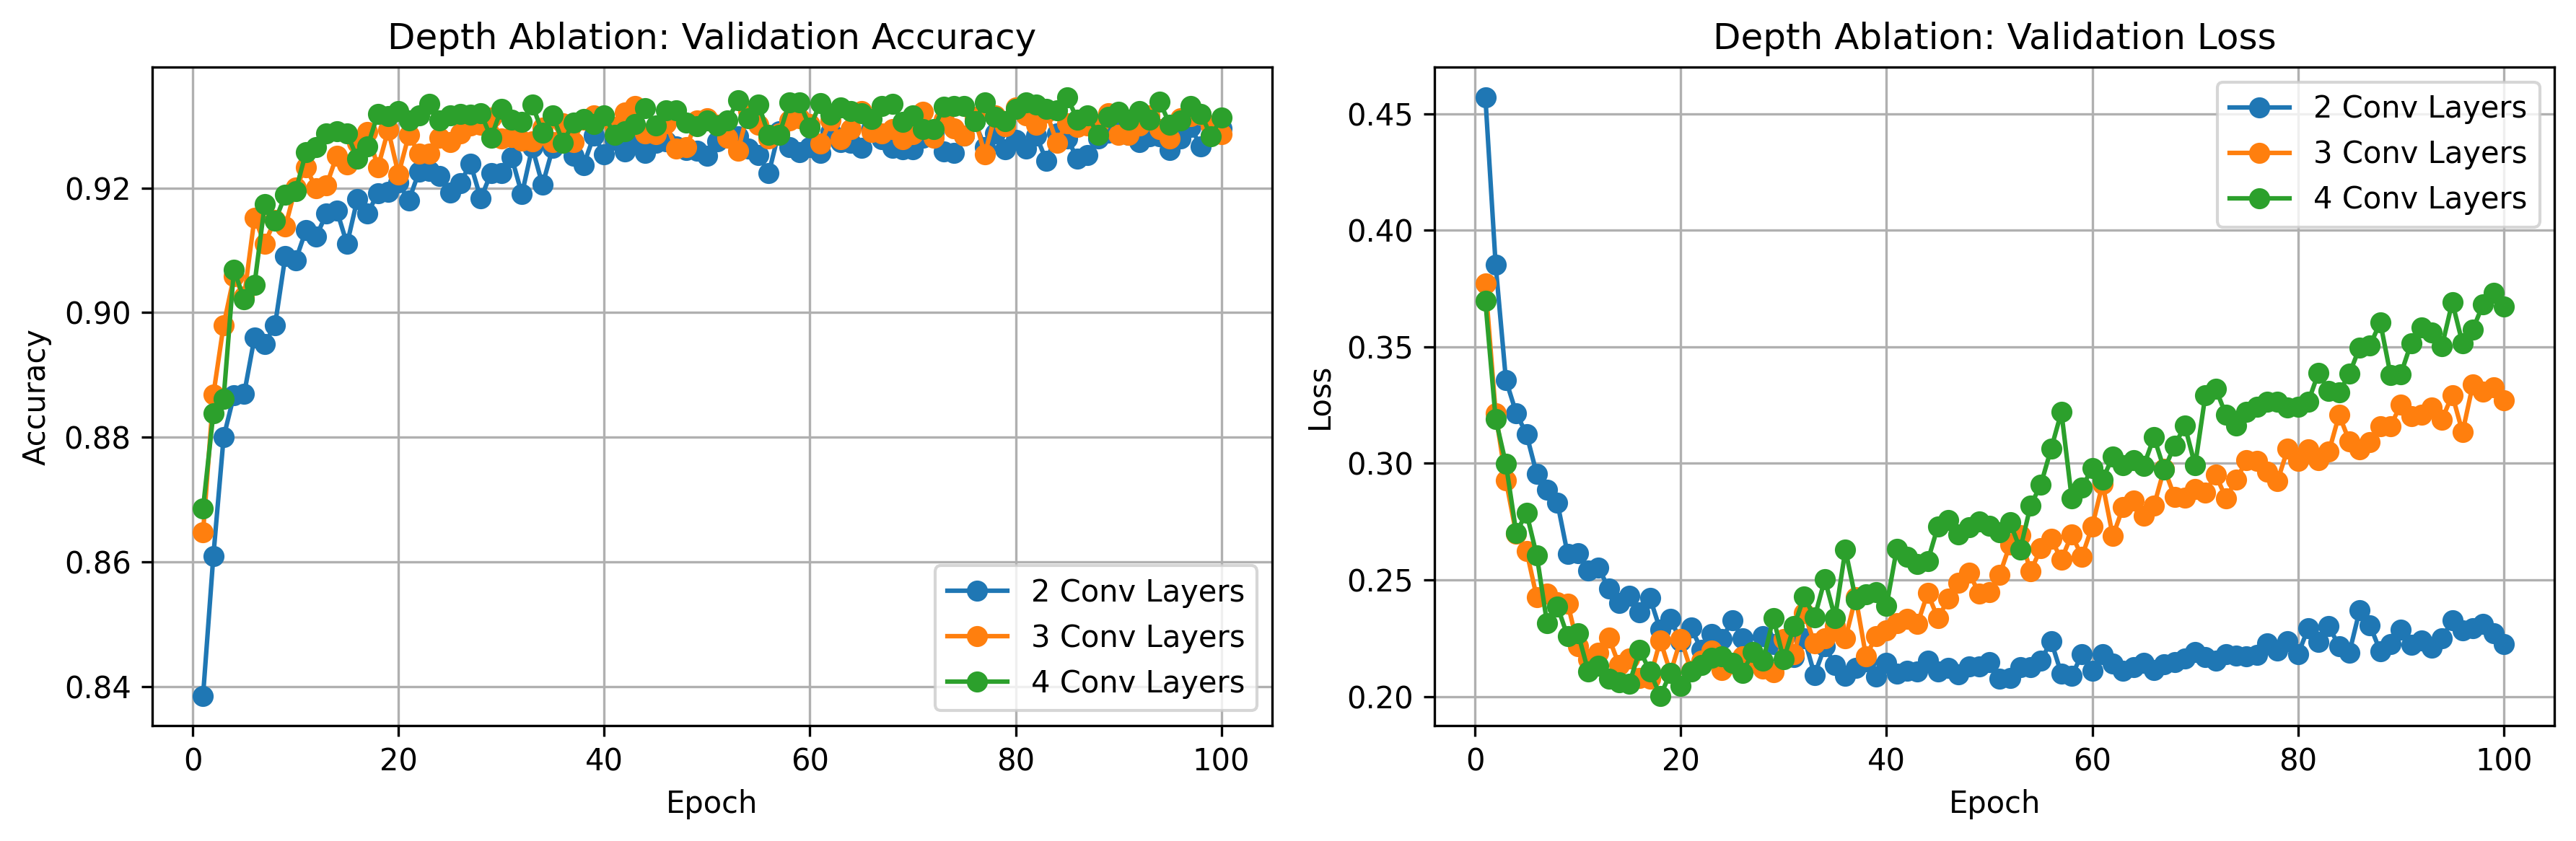
\includegraphics[width=\textwidth]{figures/depth_ablation.png}
    \caption{网络深度对验证准确率与验证损失的影响}
    \label{fig:depth-ablation}
\end{figure}

\paragraph{卷积核大小的影响}

\begin{table}[htbp]
\centering
\caption{不同卷积核大小的验证结果}
\label{tab:kernel-ablation}
\begin{tabular}{c|c|c|c}
卷积核大小 & 参数量 & 最佳 epoch & 最佳验证准确率 \\
\hline
$3 \times 3$ & 155850 & 43 & 93.31\% \\
$5 \times 5$ & 320202 & 37 & 92.91\% \\
$7 \times 7$ & 566730 & 85 & 92.67\% \\
\end{tabular}
\end{table}

表 \ref{tab:kernel-ablation} 和图 \ref{fig:kernel-ablation} 的结果与网络深度的影响类似，但区别在于，卷积核大小与准确率呈\textbf{负相关}关系，即卷积核越大，验证准确率越低；且卷积核越大，达到最优 epoch 的时间越长；相比网络深度，卷积核大小的增加对过拟合的影响更为显著。

这是因为 Fashion-MNIST 的分类依据主要在边缘、轮廓等局部结构和层次结构上；增加网络深度可以有效建模这些层次关系，而更大的卷积核不但不能建模层次结构，且更容易把局部边缘信息过早平滑掉，导致模型难以捕获细粒度的局部特征，从而降低了分类性能；卷积核的增大增强了模型的表达能力，但不是与任务匹配的增强，所以其训练更慢，过拟合也更明显。

\begin{figure}[htbp]
    \centering
    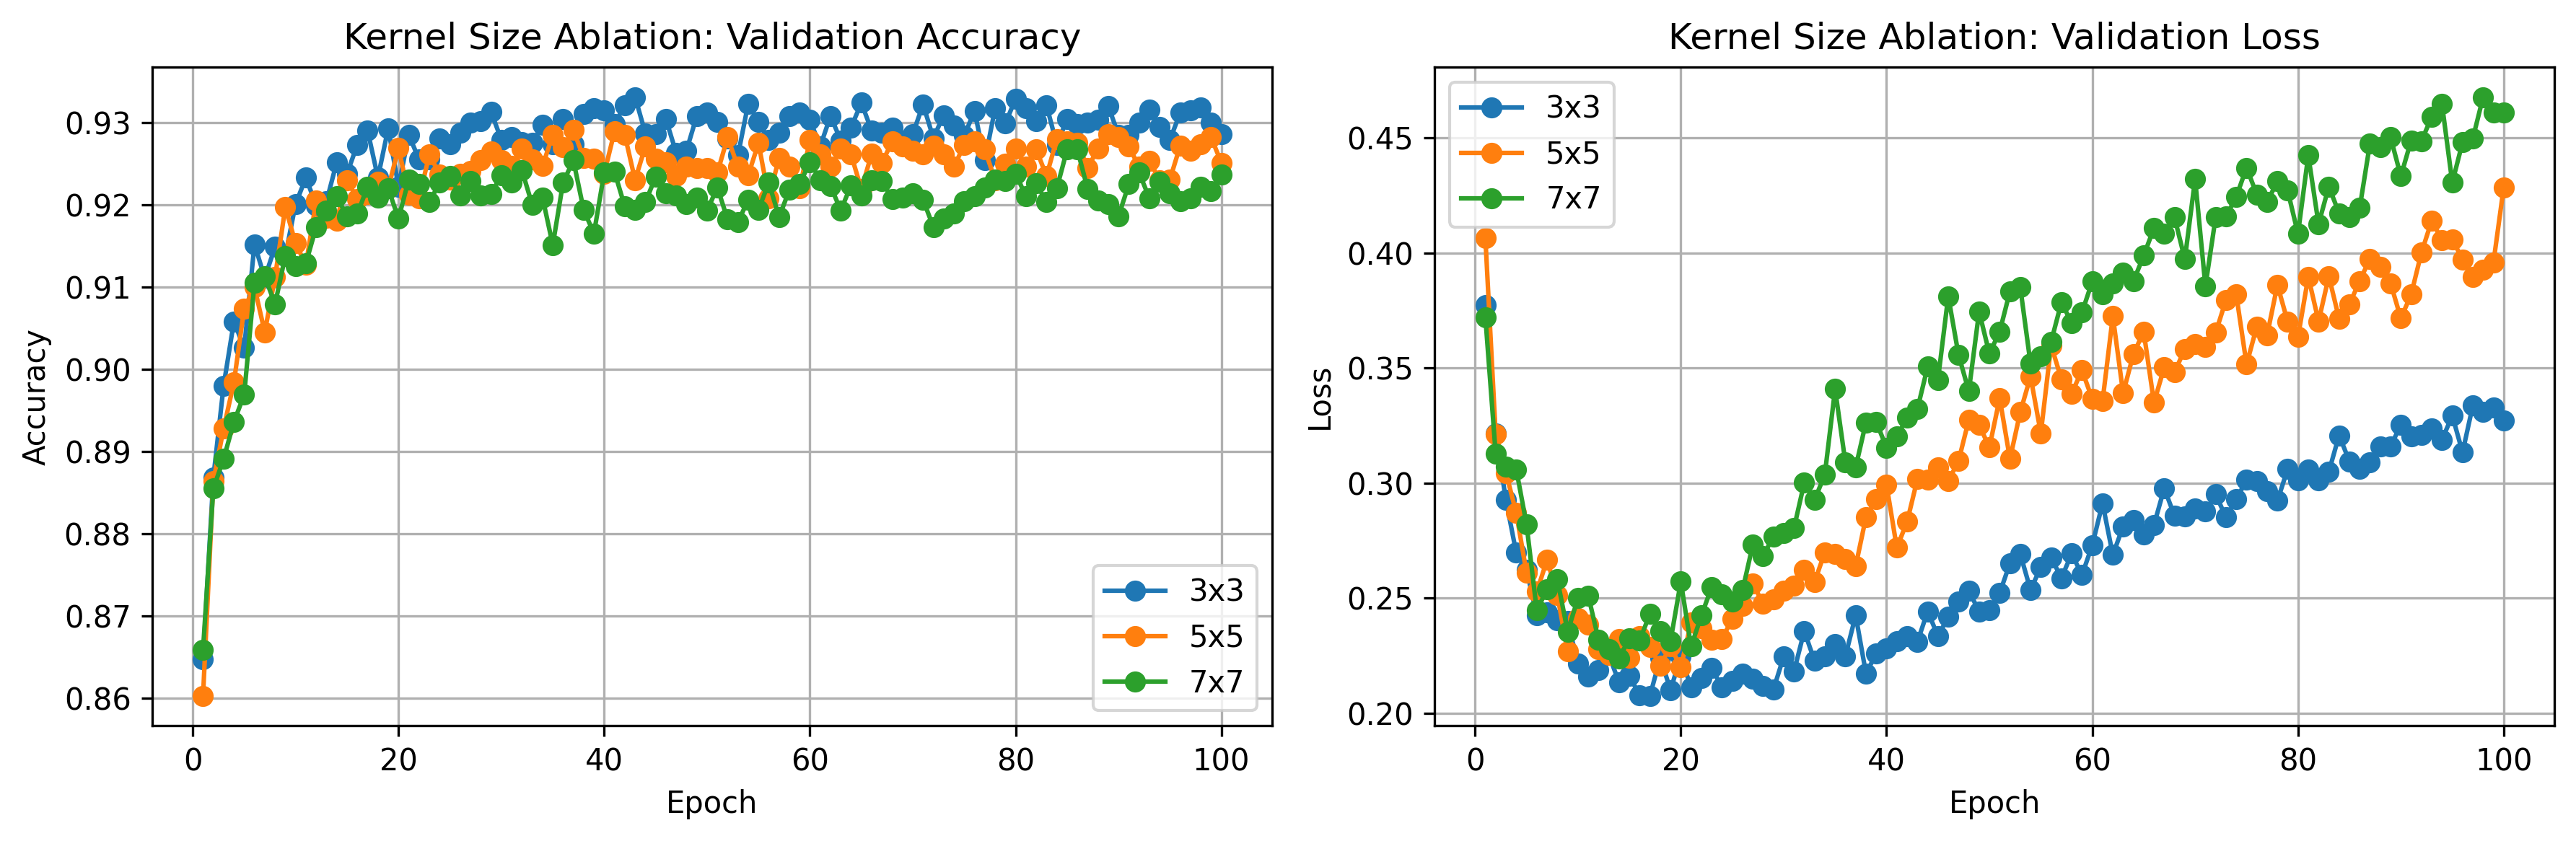
\includegraphics[width=\textwidth]{figures/kernel_ablation.png}
    \caption{卷积核大小对验证准确率与验证损失的影响}
    \label{fig:kernel-ablation}
\end{figure}

\paragraph{池化方式的影响}

\begin{table}[htbp]
\centering
\caption{不同池化方式的验证结果}
\label{tab:pooling-ablation}
\begin{tabular}{c|c|c|c}
池化方式 & 参数量 & 最佳 epoch & 最佳验证准确率 \\
\hline
Average Pooling & 155850 & 43 & 93.31\% \\
Max Pooling & 155850 & 99 & 92.66\% \\
\end{tabular}
\end{table}

在本实验中，Average Pooling 明显优于 Max Pooling，最佳验证准确率高出约 0.65 个百分点，且更早达到最优点。一个重要原因是 Fashion-MNIST 图像尺寸较小，类别之间更多依赖整体轮廓和全局形状区分，而不是非常细碎的局部纹理；Average Pooling 更倾向于保留全局信息，而 Max Pooling 会突出局部最强响应。对于这个分类任务来说，过于强调细节并不是最关键的，因此 Average Pooling 的表现更好。

\begin{figure}[htbp]
    \centering
    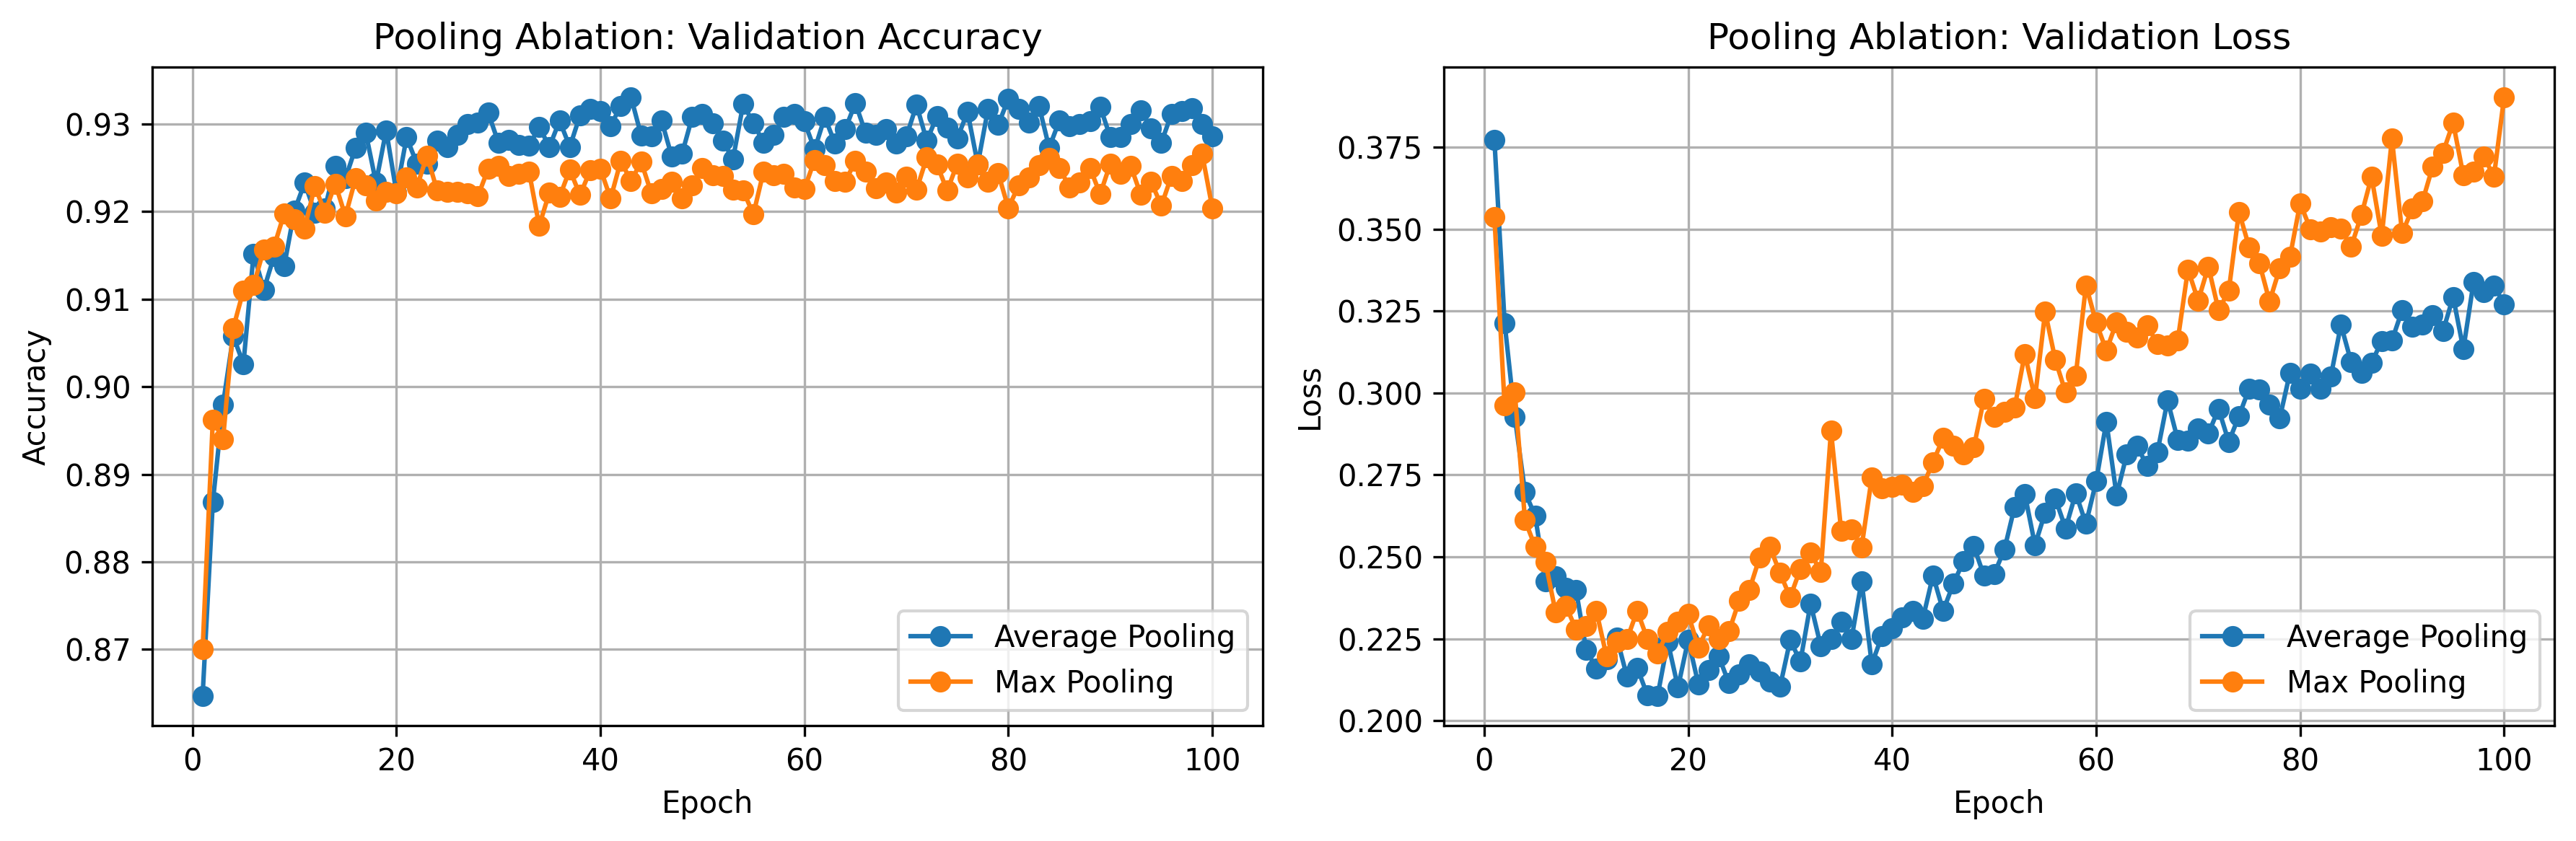
\includegraphics[width=\textwidth]{figures/pooling_ablation.png}
    \caption{池化方式对验证准确率与验证损失的影响}
    \label{fig:pooling-ablation}
\end{figure}

\paragraph{Batch Normalization 与 Dropout 的影响}

\begin{table}[htbp]
\centering
\caption{去掉 Batch Normalization 与 Dropout 的消融结果}
\label{tab:regularization-ablation}
\begin{tabular}{c|c|c|c}
设置 & 参数量 & 最佳 epoch & 最佳验证准确率 \\
\hline
Baseline & 155850 & 43 & 93.31\% \\
No BatchNorm & 155402 & 89 & 92.88\% \\
No Dropout & 155850 & 88 & 92.87\% \\
No BatchNorm or Dropout & 155402 & 95 & 92.72\% \\
\end{tabular}
\end{table}

结论上表 \ref{tab:regularization-ablation} 的结果表明，Batch Normalization 和 Dropout 都明显提高了验证准确率，并使最佳 Epoch 提前（从 89 和 88 个 epoch 提前到 43 个 epoch）；Batch Normalization 的作用主要在于加速训练；而 Dropout 更侧重于抑制过拟合，从而提高泛化能力。

图 \ref{fig:regularization-ablation} 和图 \ref{fig:regularization-ablation-train} 的训练曲线更细致地刻画了这种关系；没有 Dropout 的两组训练集上的准确率快速达到 1.0，它们是训练集上拟合最快的两组，其中有批归一化的组到达 1.0 的 epoch（第 41）比无批归一化的组（第 70）更早；但是在验证集上，它们拟合的速度却明显慢于基线，且验证 loss 曲线也表明了它们是过拟合最快的两组；

这可以从 Dropout 的原理上解释：Dropout 随机丢弃神经元的训练方式要求模型每层的数据表征都需要有一定的冗余度，所以训练收敛速度慢于不使用 Dropout 的模型；

而图 \ref{fig:regularization-ablation-train} 中明显表明，两组对比中有 Batch Normalization 层的模型的拟合速度明显快于没有的；这说明这种对均值、方差的归一化确实使训练过程更加稳定。

\begin{figure}[htbp]
    \centering
    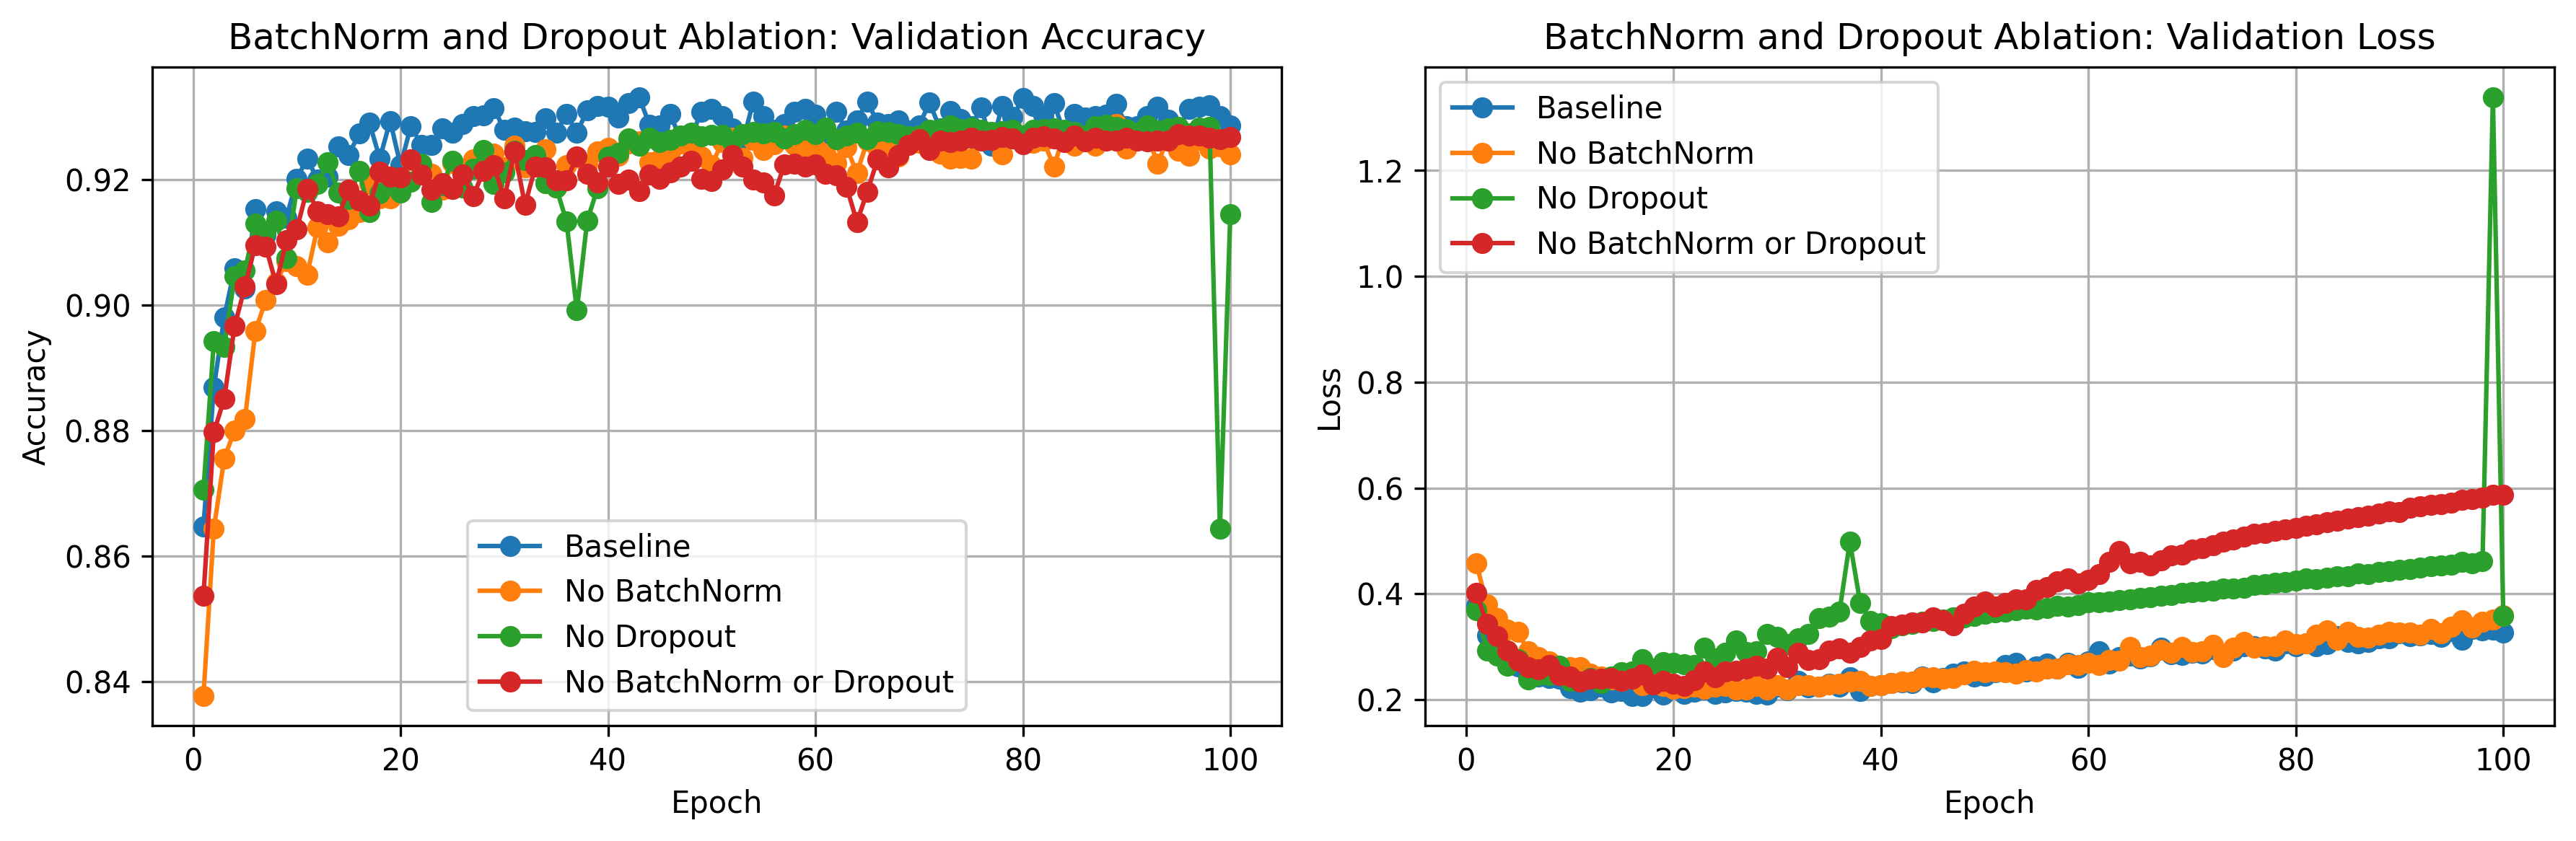
\includegraphics[width=\textwidth]{figures/regularization_ablation.png}
    \caption{Batch Normalization 与 Dropout 消融对验证准确率与验证损失的影响}
    \label{fig:regularization-ablation}
\end{figure}

\begin{figure}[htbp]
    \centering
    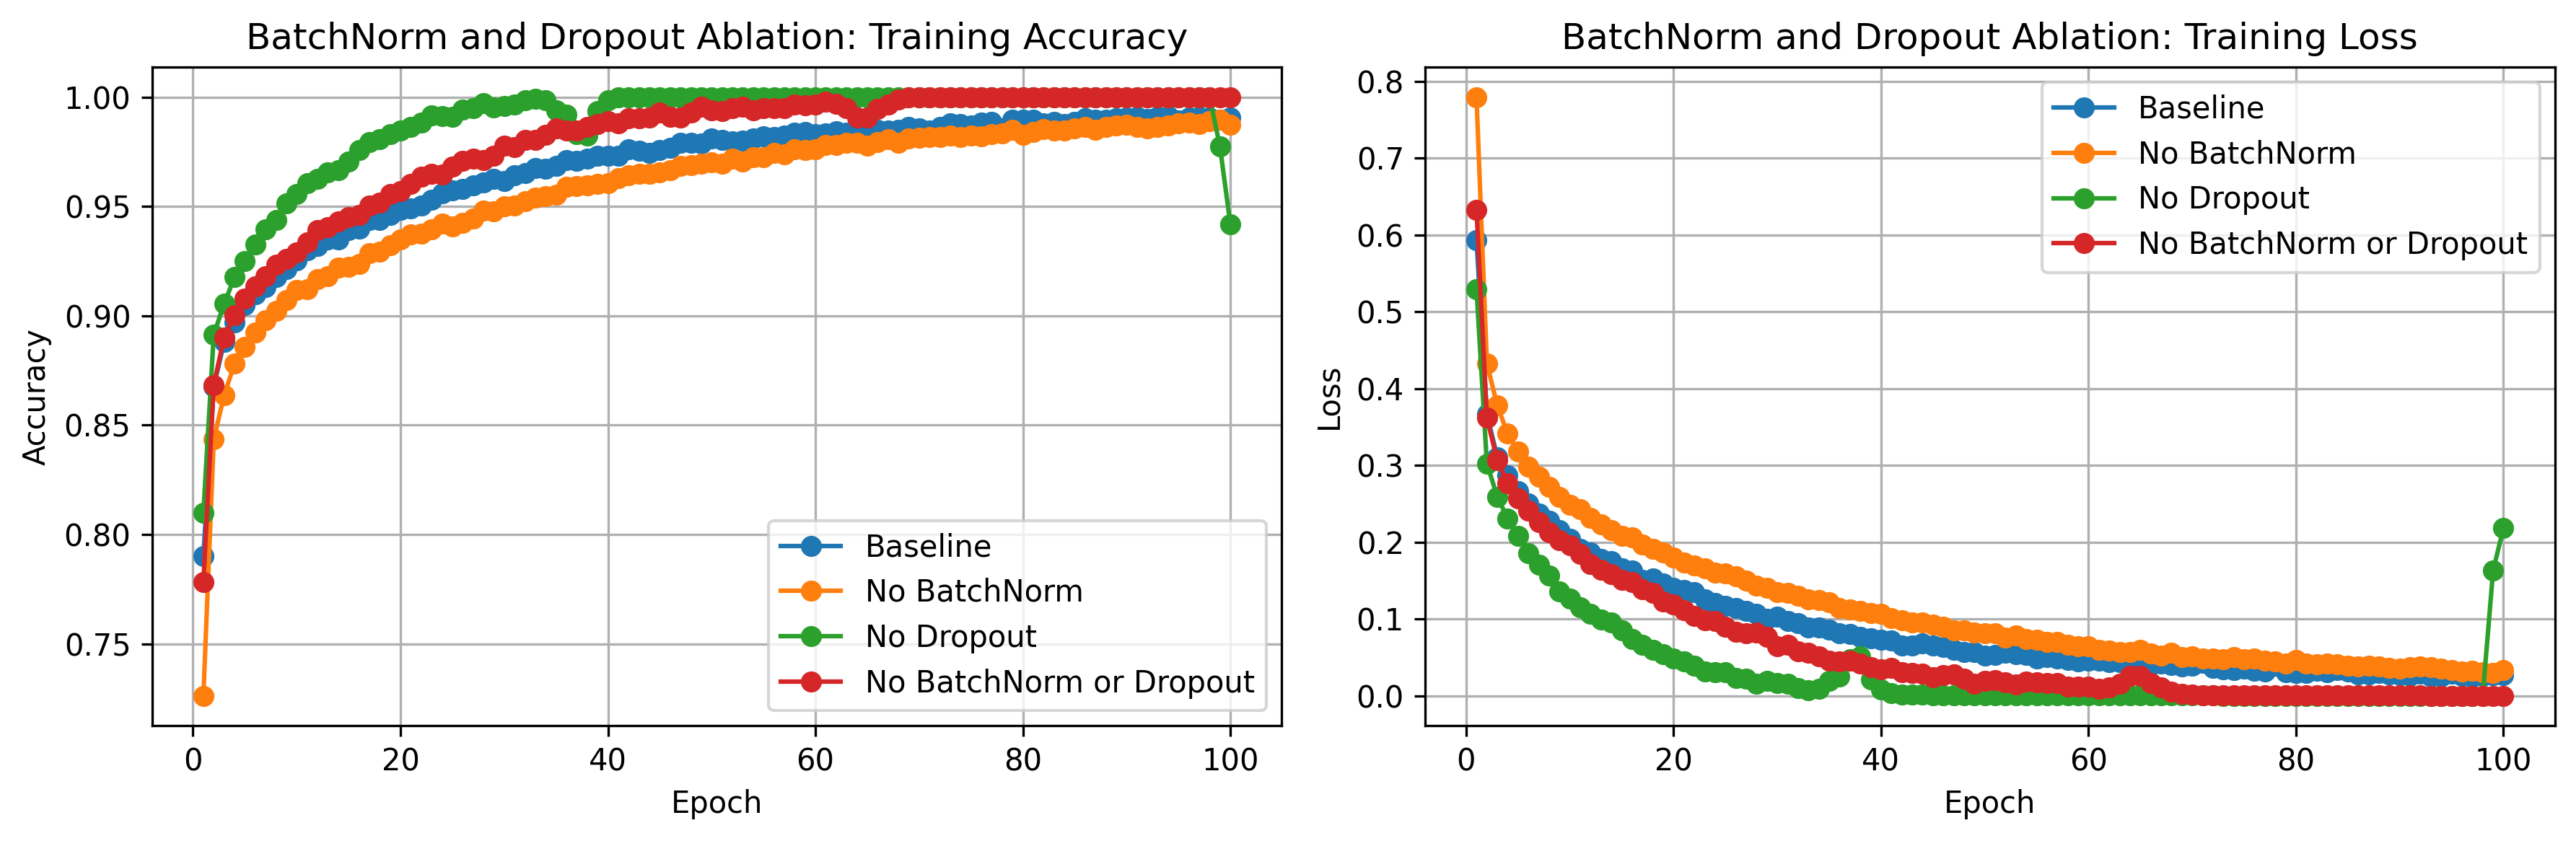
\includegraphics[width=\textwidth]{figures/regularization_ablation_train.png}
    \caption{Batch Normalization 与 Dropout 消融对训练准确率与训练损失的影响}
    \label{fig:regularization-ablation-train}
\end{figure}

\subsection{测试集分析}

\begin{figure}[htbp]
    \centering
    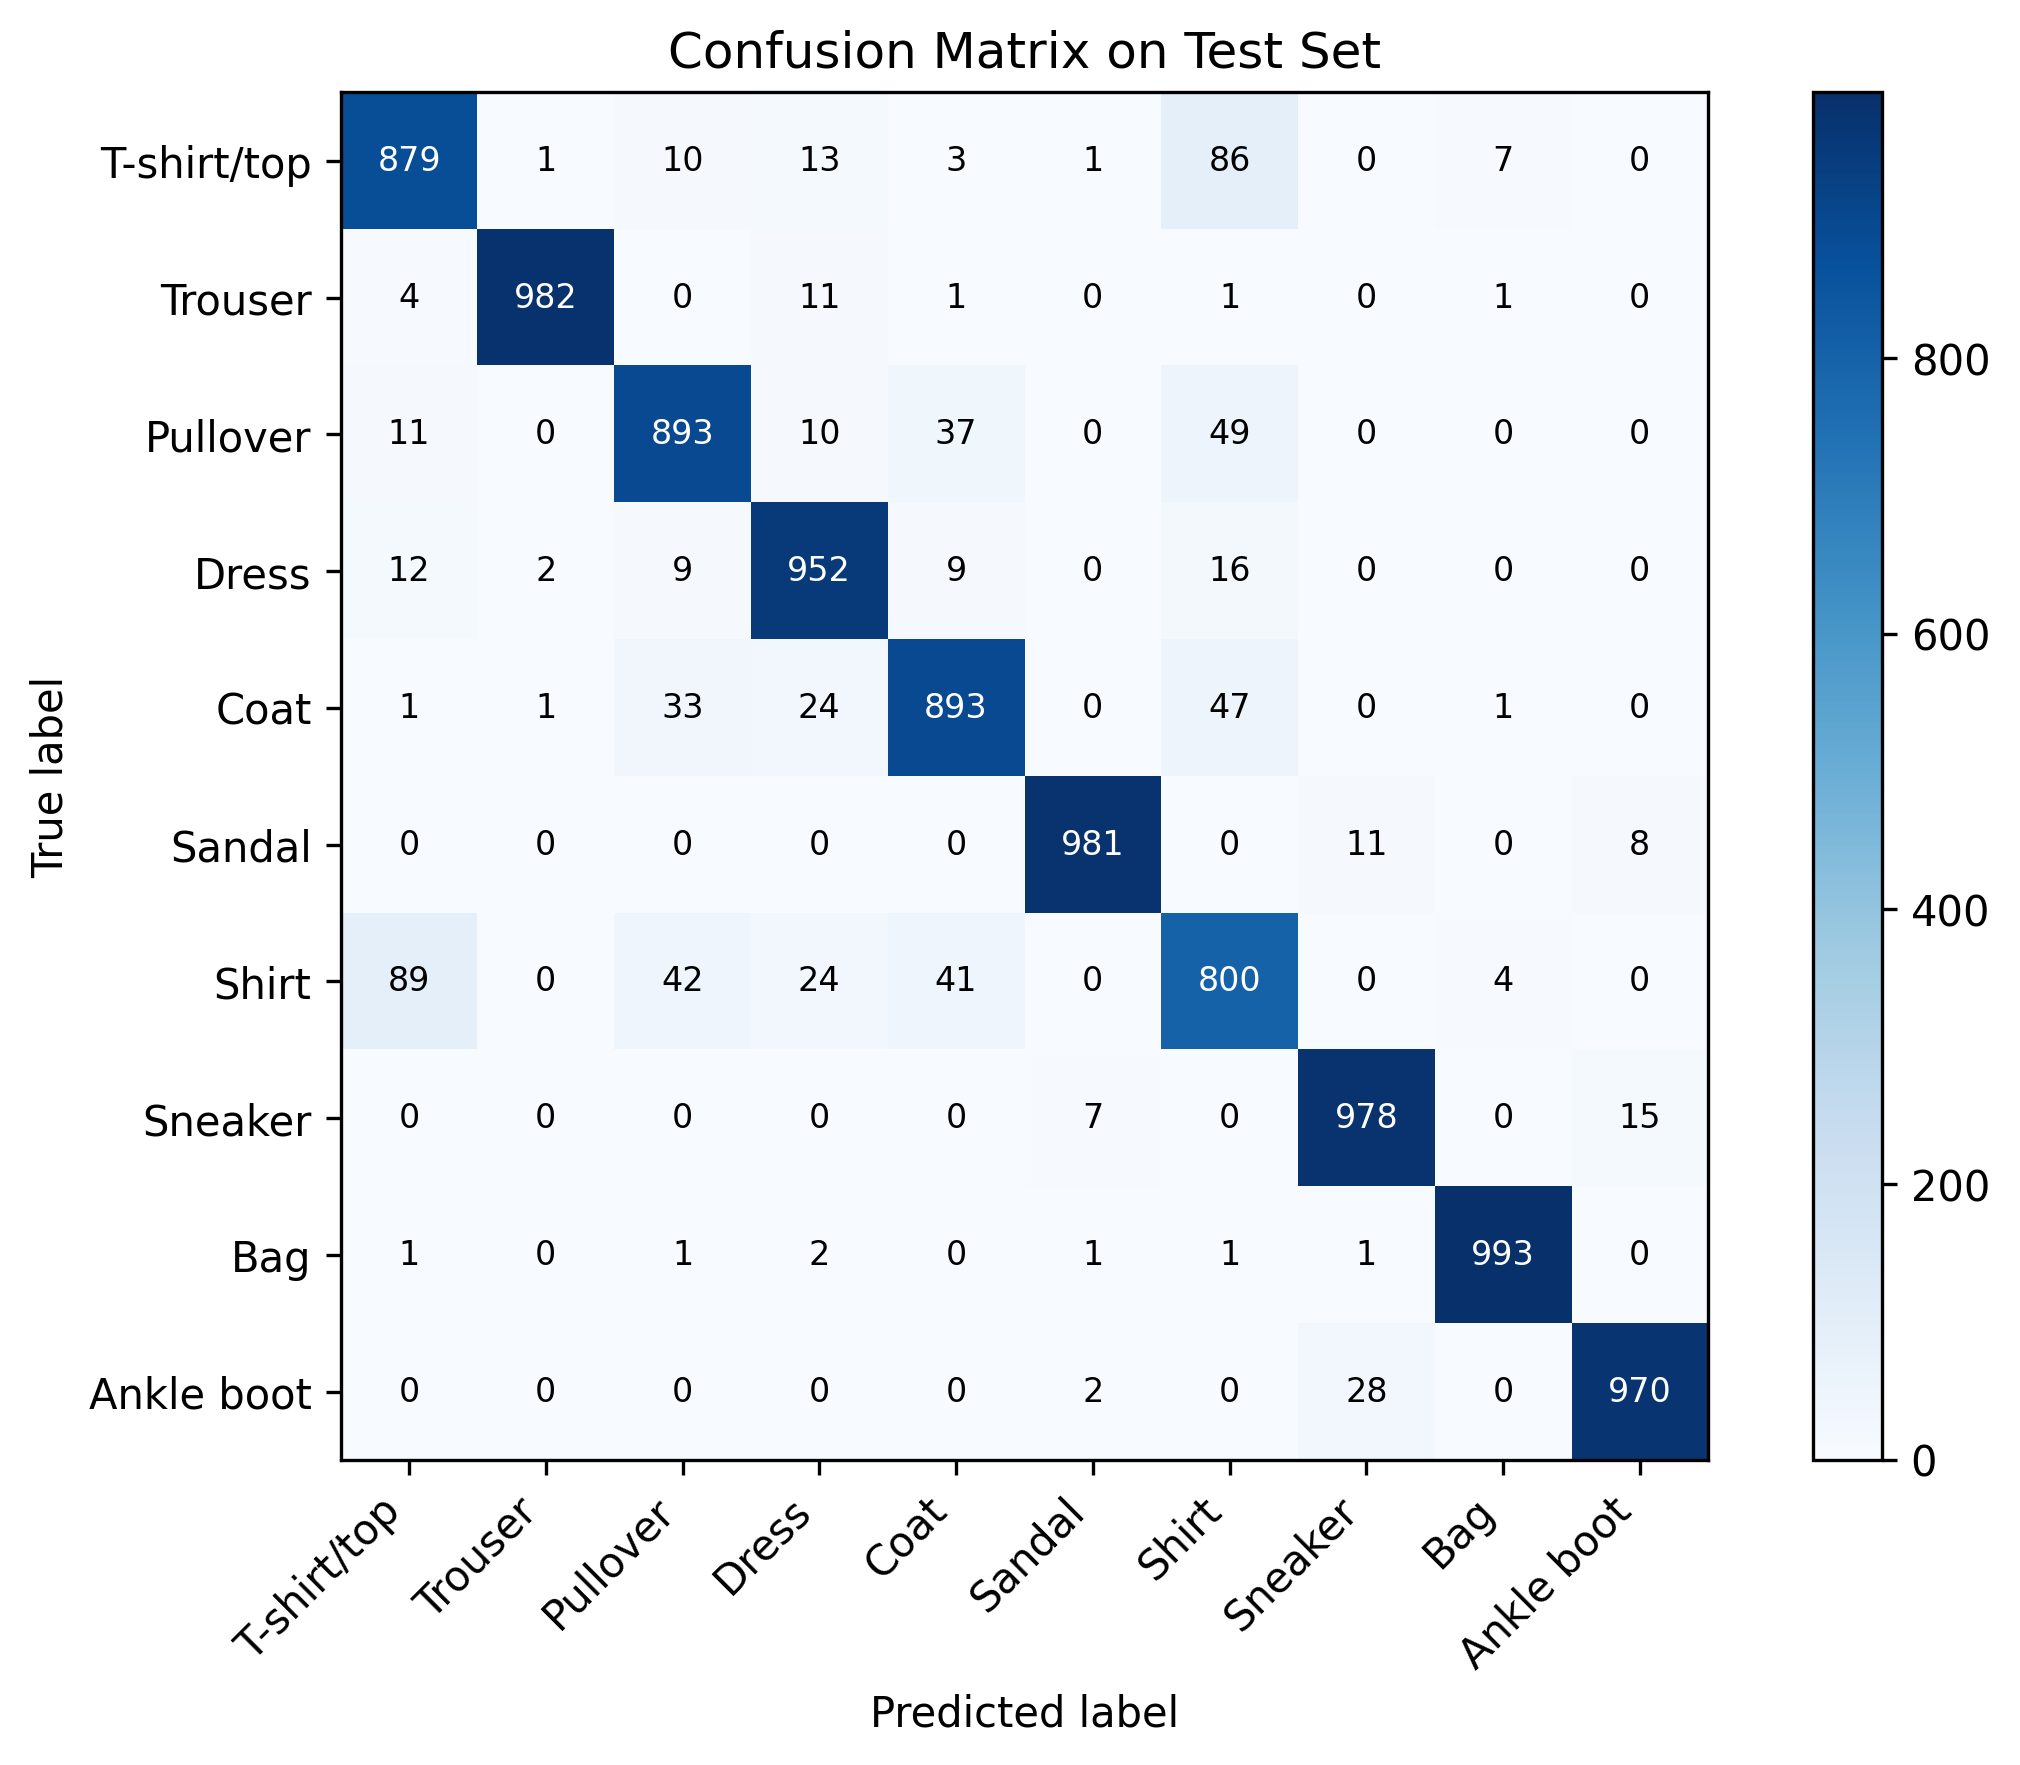
\includegraphics[width=0.82\textwidth]{figures/confusion_matrix.png}
    \vspace{-2em}
    \caption{最终模型在测试集上的混淆矩阵}
    \label{fig:confusion-matrix}
\end{figure}

\begin{figure}[htbp]
    \centering
    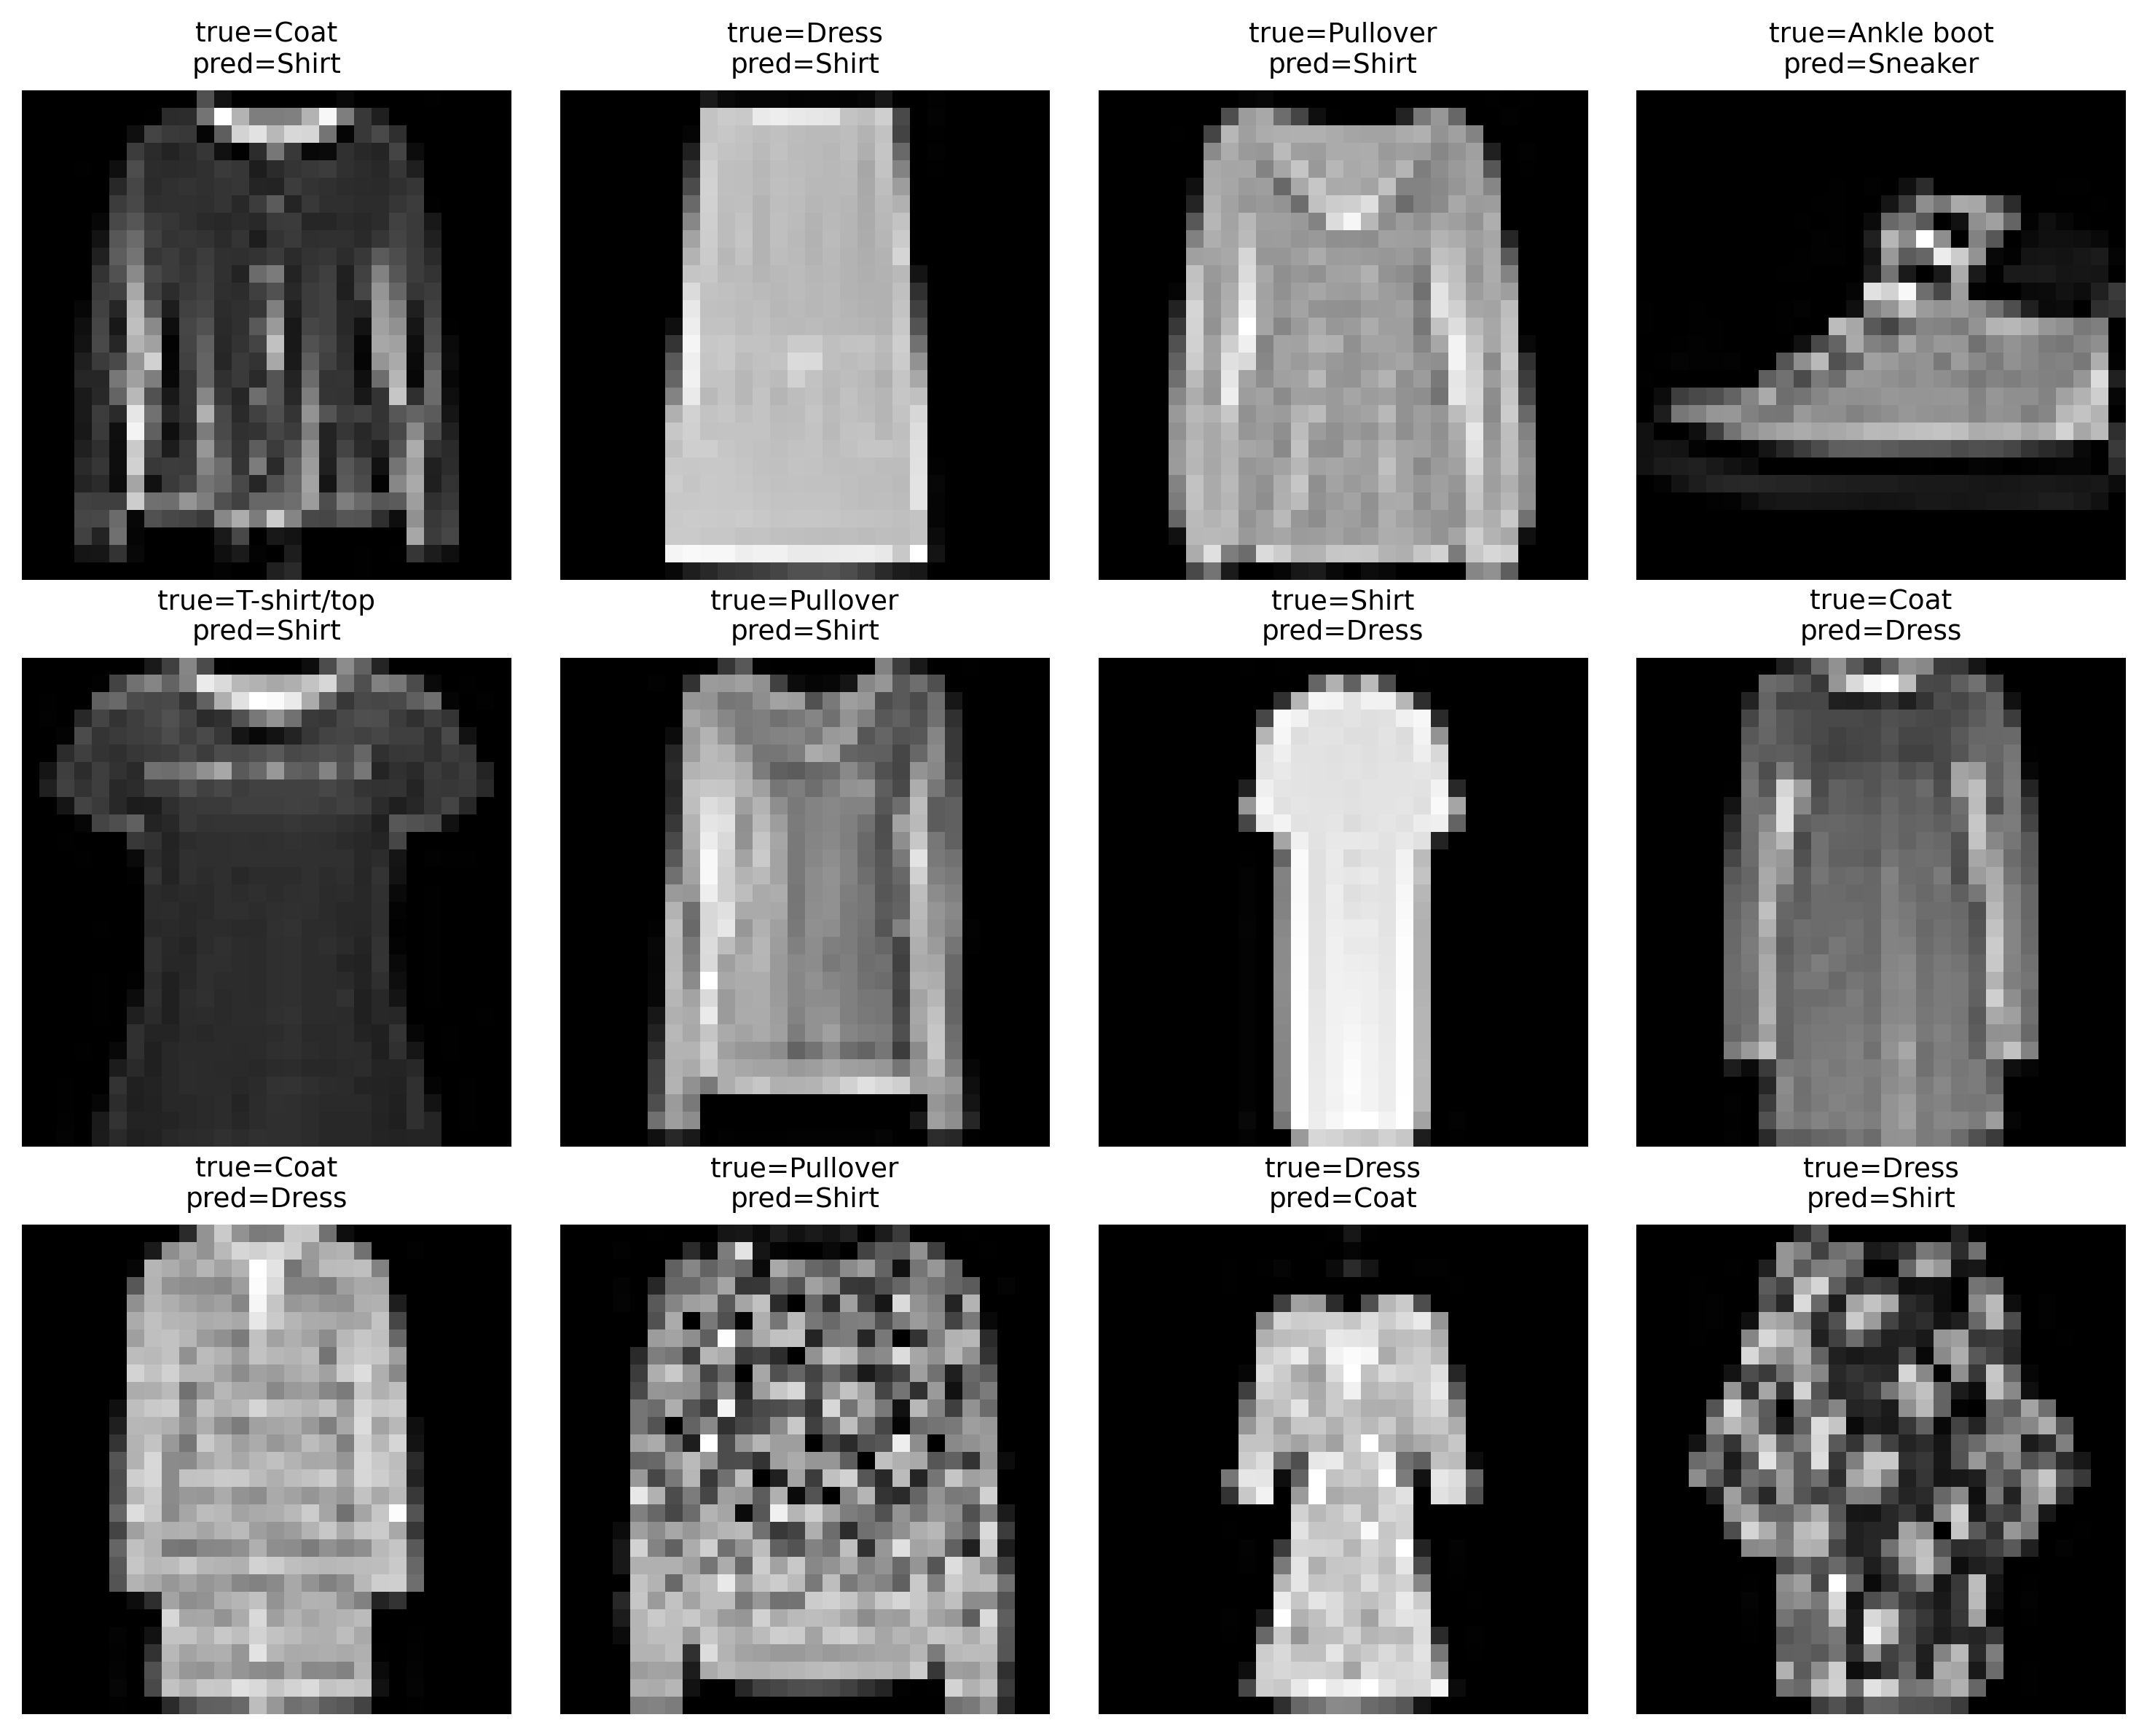
\includegraphics[width=0.82\textwidth]{figures/misclassified_examples.png}
    \caption{测试集中部分错分样本示例}
    \label{fig:misclassified-examples}
\end{figure}

从混淆矩阵可以看到，模型对 \texttt{Trouser}、\texttt{Bag}、\texttt{Sandal}、\texttt{Ankle boot} 等类别识别较稳定，而对上衣类样本的区分最困难。如图 \ref{fig:misclassified-examples}，最终一次测试中，最常见的错误包括：

\begin{itemize}[noitemsep]
    \item \texttt{Shirt} 被分成 \texttt{T-shirt/top}：89 次；
    \item \texttt{T-shirt/top} 被分成 \texttt{Shirt}：86 次；
    \item \texttt{Pullover} 被分成 \texttt{Shirt}：49 次；
    \item \texttt{Coat} 被分成 \texttt{Shirt}：47 次；
    \item \texttt{Shirt} 被分成 \texttt{Pullover}：42 次。
\end{itemize}

这些错分基本符合数据集本身的视觉特点：\texttt{T-shirt/top}、\texttt{Shirt}、\texttt{Pullover}、\texttt{Coat} 在灰度图中主要依赖轮廓和袖口形状区分，而这些差异较细微；鞋类中的 \texttt{Sneaker} 与 \texttt{Ankle boot} 也有相似的边缘结构，因此在低分辨率下容易混淆。相比之下，裤子、包等类别的外形更稳定，故准确率更高。

\section{疑难点}

本次实验的疑难点主要集中在性能问题上：我与同学对比了各自的代码在 NVidia GPU 上的运行时间，发现在 \verb|DataLoader| 同时设置 \verb|num_workers=0|，且训练模型大小相同的时候，我的代码 GPU Utilization 略低于我比较的代码；而我把 DataLoader 改成 \verb|num_workers=4| 后，这个 GPU Utilization 和他的实现就没有明显区别。

目前我还没有找出这个问题的根本原因；但是我大致可以确认，该实验的性能瓶颈不在 GPU 上，而在于 GPU 与主板间的 PCIe 传输或者 CPU 内存与总线间的传输上；因为 Apple MPS 间的训练速度与模型尺寸明显成比例，但是 NVidia GPU 上训练速度受模型尺寸的影响不大。

\section{结论}

本实验完成了基于 CNN 的 Fashion-MNIST 分类任务，并围绕网络深度、卷积核大小、池化方式以及 Batch Normalization / Dropout 设置四项因素进行了对比分析。主要结论如下：

\begin{itemize}[noitemsep]
    \item 深度方面，网络从 2 层加深到 4 层仍有稳定提升，最终 4 层卷积模型取得了全局最优结果；
    \item 卷积核方面，$3 \times 3$ 小卷积核表现最好，更大的卷积核带来了更多参数，但没有带来更好的泛化；
    \item 池化方式方面，Average Pooling 明显优于 Max Pooling；对于尺寸较小的 Fashion-MNIST 图像，保留全局轮廓信息比强调局部极值更重要；
    \item Batch Normalization 让训练更快，Dropout 则有效减轻过拟合；不带 Dropout 的模型甚至在训练集上达到 1.0000 的准确率，但验证集表现反而下降；
    \item 最终的 4 层卷积模型在测试集上取得了 $93.21\%$ 的分类准确率，说明适度加深且训练稳定的 CNN 已能较好完成 Fashion-MNIST 分类。
\end{itemize}

综合来看，Fashion-MNIST 更需要“与任务匹配的结构”而不是单纯堆大模型：较小卷积核、Average Pooling、Batch Normalization 与 Dropout 的组合能提供更好的训练稳定性和泛化能力；在此基础上适度增加深度，能够进一步提升分类性能。

\end{document}
